\chapter{Evaluation and Results}

This chapter evaluates whether the implemented system preserves the evidence boundary defined in Chapters 2 and 3. The protocol separates logical conformance, hostile input handling, temporal state, pack identity, Android packaging, physical interaction, and visual communication. Results are reported before interpretation so that a positive engineering outcome is not silently promoted into a legal, population, or store-approval claim.

\section{Evaluation Overview and Headline Results}

The evaluation separates seven evidence layers: (1) source and specification conformance; (2) deterministic and adversarial rule behaviour; (3) formal properties and curated mutation detection; (4) corpus-scale static and workflow evidence; (5) assembled-package and physical-device integration; (6) rendered UI and accessibility-oriented inspection; and (7) independent human and legal validation. Layers one to six contain the bounded observations reported below. Layer seven remains \texttt{NOT\_RUN}. This separation prevents a passed unit test from being reported as device reliability, human comprehension, or legal validity. Historical receipts remain under \RepoTree{testing-report/}; the final OPPO package and interaction receipt is retained under \RepoTree{testing-report/real-device-9-8-finalize-v1.15.0/}.

\subsection{Evidence Objects, Units, and Denominators}

Table~\ref{tab:evidence-objects} states the unit of analysis that each evidence object supports, and it exists to make unit mixing visible. Counts expressed in different units---seeded logical cases, generated permutations, executed assertions, matched rule events, APK files, package identities, workflow runs, device runs, interface observations, and review-packet items---are not summed anywhere in this thesis, and no two rows may be added together. Where the relation between two objects is not established by a recorded mapping, they are reported separately rather than as one funnel. In particular, the \FDroidCensusN{}-APK static census and the \DevicePackagesN{}-package device denominator are separate populations, and no verified mapping from the former to the latter is claimed.

\begin{table}[H]
\centering
\caption{Evidence objects, recorded scale, unit of analysis, and what each can support}
\label{tab:evidence-objects}
\scriptsize
\setlength{\tabcolsep}{3pt}
\begin{tabular}{>{\raggedright\arraybackslash}p{0.14\textwidth}>{\raggedright\arraybackslash}p{0.23\textwidth}>{\raggedright\arraybackslash}p{0.16\textwidth}>{\raggedright\arraybackslash}p{0.20\textwidth}>{\raggedright\arraybackslash}p{0.19\textwidth}}
\toprule
Evidence object & Recorded scale & Unit of analysis & Supports & Does not support \\
\midrule
Seeded logical campaign & 1{,}000 cases; $(TP,TN,FP,FN)=(800,200,0,0)$ & generated case against a specified oracle & conformance of the engine to the published threshold model & real infringement detection or a population error rate \\
Permutation fixture & six events; 720 permutations & permutation of one effective event multiset & order independence within the stated retention model & global order independence for all states or truncation policies \\
Stress campaign & \StressCorpusN{} corpora; \StressRestartN{} restart; \StressMalformedN{} malformed; \StressAssertionsN{} assertions; \StressRuleMatchesN{} rule matches & generated input, executed assertion, matched rule event & reproducibility and fail-closed invariants on a fixed generated distribution & independent samples, population rates, or performance benchmarks \\
Registered properties and mutants & 9 properties; 9 registered non-equivalent weakenings; 9 reported detections & property and registered weakening & sensitivity to the registered semantic weakenings & a complete mutation score or absence of unmodelled defects \\
F-Droid static census & \FDroidCensusN{} APKs; \FDroidSensitiveN{} sensitive-permission; \FDroidSensitiveNetworkN{} sensitive-plus-network; \FDroidSensitiveBackgroundN{} sensitive-plus-background; \FDroidMultiProcessN{} multi-process & APK file with static manifest and DEX-reference features & composition and processing of the selected corpus & runtime flows, lawful basis, or commercial-store representativeness \\
Device workflow receipts & \DevicePackagesN{} package identities; \CompletedWorkflowsN{} completed; \FailedDeviceWorkflowsN{} retained failures & package identity and workflow run & execution results for this device and fixed procedure & \DevicePackagesN{} devices, \DevicePackagesN{} users, or a complete usage path \\
Recorded failure classes & 26 installer timeouts; 2 no-launchable-activity; 1 package-manager rejection; 1 pre-existing-package protection & retained failure record & the recorded terminal state of the failed runs & causal explanations that were not recorded \\
Post-launch PSS measurements & \PssObservedN{} available of \CompletedWorkflowsN{} completed & measurement on one completed workflow & a descriptive distribution for the measured subset & zero missingness, a memory-leak claim, or a population distribution \\
End-to-end timing measurements & \TimingObservedN{} available of \CompletedWorkflowsN{} completed & recorded workflow duration & the duration of the recorded workflow & per-decision latency of the review engine \\
OEM permission-interface observations & 48 observed; 155 not observed; \FailedDeviceWorkflowsN{} unavailable for failed runs; 31 deny-only notification actions & package run and interface action & the recorded interface boundary behaviour & 31 additional independent applications, or grants and actual use \\
FlowDroid evidence set & \FlowDroidReceiptsN{} receipt; \FlowDroidXmlArtifactsN{} XML artifacts & tool invocation & missing-output handling and adapter interoperability & a successful real-application comparison or algorithm superiority \\
Regulation-mapping review packet & 13 atomic items; independent review not run & review item & preparation of a review instrument & legal approval or inter-rater agreement \\
Single-device release record & one build identity, one device, one interaction interval & installed build on one device & an implementation witness for the recorded scope & cross-OEM behaviour, long-run stability, or accessibility conformance \\
\bottomrule
\end{tabular}
\end{table}

Table~\ref{tab:rq-result-map} then locates the results reported later in this chapter against the four research questions, so that a reader can check that every question receives an answer and that no answer is assembled from a section that does not address it.

\begin{table}[H]
\centering
\caption{Research questions and the sections that answer them}
\label{tab:rq-result-map}
\scriptsize
\setlength{\tabcolsep}{4pt}
\begin{tabular}{>{\raggedright\arraybackslash}p{0.05\textwidth}>{\raggedright\arraybackslash}p{0.42\textwidth}>{\raggedright\arraybackslash}p{0.42\textwidth}}
\toprule
RQ & Principal results in this chapter & Evidence objects used \\
\midrule
RQ1 & Deterministic corpus interpretation; adversarial input results; temporal and replay results; temporal correctness and restart evidence & seeded cases; boundary fixtures; malformed inputs; restart comparisons \\
RQ2 & Accountability and presentation results; visual review method; device interaction protocol & policy fixtures; dashboard projection; UI hierarchy; screenshots \\
RQ3 & Regulation-pack results; cross-pack rejection; retained pack identity in findings; mapping-review preparation & two registered packs; pack-switch fixtures; 13-item review packet \\
RQ4 & F-Droid static census; device workflow denominators and failures; measurement availability; FlowDroid missing output; evidence-object table & corpus records; device receipts; missing measurements; tool receipt \\
\bottomrule
\end{tabular}
\end{table}

\subsection{Source and Rule Verification}

The complete application passed \texttt{tsc --noEmit} and ESLint. The compliance sources were compiled before execution, preventing stale generated JavaScript from being treated as current evidence.

A fixed-seed logical campaign generated 1,000 cases. Eight hundred were expected review signals and 200 were below-threshold controls. The observed confusion matrix was

\begin{equation}
(TP,TN,FP,FN)=(800,200,0,0),
\end{equation}

which gives precision and recall of 1.0000 against the specified oracle. The oracle and engine implement the same published threshold model; this is a conformance and regression result, not an independent estimate of real-world infringement detection. Zero observed errors do not establish a zero population error rate.

Extended suites passed for unsafe types and integers, malformed context, unknown source, permission-key mutation, temporal overlap, adjacency, replay, retention, simulator isolation, dashboard presentation, missing-context disclosure, and regulation-pack identity. The tests confirm the enumerated boundaries. They cannot establish correctness for telemetry the application never receives or for legal interpretation outside the fixtures.

\subsection{Release Build and Manifest Verification}

Gradle completed \texttt{assembleRelease} and \texttt{bundleRelease} with target SDK 36 in the recorded build workflow. The 9 August receipt contains binary hashes for an earlier candidate and is retained as historical build-pipeline evidence; those hashes are not attributed to release \PrivacyLensVersion{}. Two published revisions identify the source line used here: the frozen research baseline is branch \texttt{8-22} at commit \RepoCommitLink{727056c4b29065a4c21ab9bc291c85ca8fa93d5f}{727056c4}, and the mature candidate is branch \texttt{8-24} at commit \RepoCommitLink{225b03476dd863ee79caf56d96f84d52a379daa5}{225b0347}. An undated ``research freeze'' label is avoided because the repository records branch-and-commit identities rather than a single freeze date. The 8 September finalisation rebuilt the release APK and AAB from that source line and recorded their hashes; Play signing and store delivery remain external owner actions.

The reconciled release manifest contained wake lock, boot rescheduling, foreground service, and an application-scoped dynamic-receiver signature permission. Internet, network-state, and legacy external-storage read/write declarations were absent. APK inspection and the installed-package dump reported the same set, with no dangerous runtime permission requested or granted. Android backup was disabled in the application declaration.

\subsection{Physical-Device Evaluation}

The release APK was installed by ADB on one OPPO PERM00 ARM64 device. The installed package reported \texttt{com.zhihengzhang.privacylens}, versionName \PrivacyLensVersion{}, versionCode 16, minSdk 24, and targetSdk 36. Launcher cold start and the overview--findings--settings path succeeded in the bounded 8 September finalisation interval. The filtered crash buffer contained no matching fatal record after that path. This is an observation for one installed build and interval, not a long-run crash-rate estimate.

The three primary destinations rendered at the device's captured application resolution. Coordinate-driven exploration initially appeared to show a navigation-target problem because the physical display and captured application coordinate spaces differed. A bounded coordinate sweep and UI-tree inspection identified the offset; subsequent navigation and custom bottom-bar interaction succeeded. This calibration episode is retained because it demonstrates why raw ADB coordinates must not be interpreted without the target's current window geometry.

The controlled demonstration completed a 50-record synthetic workflow. The populated overview displayed four review items, zero evidence gaps, two no-concern items, and descriptive precision and recall of 100\% for the simulator's known labels. The Findings screen marked the source as synthetic and displayed the EU GDPR pack. These values validate the demonstration path only; they are not device-observation accuracy.

\subsection{Verified Open-Source App-Store Execution}

To test the engineering workflow beyond the project APK, a separate authorised corpus was constructed from the official F-Droid repository. This is an \emph{open-source app-store} corpus, not a closed-source commercial-store sample. The final hash-pinned static census contains \FDroidCensusN{} APKs; the device subset and its exclusion boundary are separately receipt-owned. The corpus boundary and the final static census are recorded under \RepoTree{testing-report/fdroid-open-store-2026-08-22/}, together with the device-batch aggregates. The upstream F-Droid catalogue snapshot from which the corpus was drawn is not part of the published artifact, so corpus composition is reported here from the census itself rather than from a catalogue file. Figure~\ref{fig:census-composition} shows the composition of that corpus, and the overlap warning in its caption is deliberate.

\begin{figure}[H]
\centering
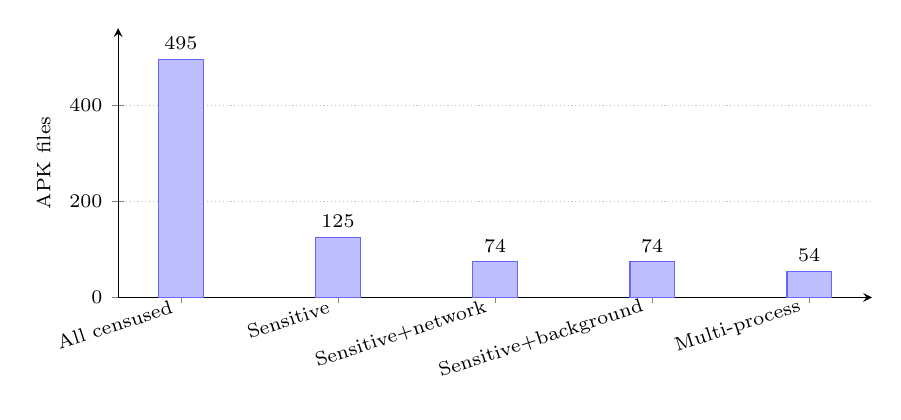
\begin{tikzpicture}
\begin{axis}[
  width=0.92\textwidth, height=5.0cm,
  ybar, bar width=16pt,
  ymin=0, ymax=560,
  ylabel={\scriptsize APK files},
  symbolic x coords={All censused, Sensitive, Sensitive+network, Sensitive+background, Multi-process},
  xtick=data,
  x tick label style={font=\scriptsize, rotate=18, anchor=east},
  y tick label style={font=\scriptsize},
  ymajorgrids, grid style={densely dotted},
  nodes near coords, every node near coord/.append style={font=\scriptsize},
  axis lines=left, enlarge x limits=0.10,
]
% Values match generated-results.tex macros: FDroidCensusN=495,
% FDroidSensitiveN=125, FDroidSensitiveNetworkN=74,
% FDroidSensitiveBackgroundN=74, FDroidMultiProcessN=54.
% Literal coordinates are used because pgfplots cannot parse these macros here.
\addplot[fill=blue!25, draw=blue!60] coordinates {
  (All censused,495)
  (Sensitive,125)
  (Sensitive+network,74)
  (Sensitive+background,74)
  (Multi-process,54)
};
\end{axis}
\end{tikzpicture}
\caption{Static features of the hash-pinned F-Droid corpus. The categories overlap: the sensitive-permission counts are subsets of the censused set, and the network and background counts are not disjoint from one another, so the bars must not be added together.}
\label{fig:census-composition}
\end{figure}

The physical-device runner processed \DevicePackagesN{} distinct package identities over three non-overlapping receipts. It completed \CompletedWorkflowsN{} workflows comprising install, launch, force-stop, and uninstall, and retained \FailedDeviceWorkflowsN{} failures: 26 installer timeouts, two no-launchable-activity cases, one package-manager rejection, and one pre-existing-package protection. No removal failure was observed. The protection is important: a package present before the runner reaches it is neither replaced nor uninstalled, even on the controlled test device.

A final \FDroidCensusN{}-APK static Manifest and DEX-reference census completed without a static failure. It found \FDroidMultiProcessN{} declared multi-process applications, \FDroidSensitiveBackgroundN{} sensitive-permission-plus-background-execution review signals, and \FDroidSensitiveNetworkN{} sensitive-permission-plus-network review signals. These results establish corpus diversity and static review coverage only. They do not establish a runtime source-to-sink flow, controller purpose, lawful basis, necessity, or GDPR infringement. The information-flow model was instead stress-tested through controlled adversarial graphs: obfuscated node identifiers, reflection edges, dynamic runtime-permission evidence, and Binder/Worker cross-process paths preserve a typed review prompt; malformed graph edges fail closed. Its $(TP,FP,TN,FN)=(3,0,1,0)$ result is a fixture-oracle conformance result, not a field estimate.

The final aggregate collected post-launch memory for \PssObservedN{} non-overlapping packages: median PSS was \num{\DevicePssMedianKb} KB with an interquartile range from \num{\DevicePssQOneKb} to \num{\DevicePssQThreeKb} KB. End-to-end workflow time was observed for \TimingObservedN{} completed workflows: the median was \num{\DeviceTimingMedianMs} ms with an interquartile range from \num{\DeviceTimingQOneMs} to \num{\DeviceTimingQThreeMs} ms. Memory was unavailable for 105 of \CompletedWorkflowsN{} completed workflows and timing for 102; these are retained as missing telemetry rather than converted to zero. Across all receipts, the OEM runtime-permission UI was observed but not granted in 48 package runs, not observed in 155, and unavailable for the \FailedDeviceWorkflowsN{} failed runs. A catalog-bound observer separately dismissed 31 exact notification prompts by selecting only the denial control, never a grant control. This shows that the runner preserved the dynamic-permission prompt boundary; it does not establish that each application requested, received, or used a permission. Likewise, the real-app corpus has no independent legal ground truth, so precision, recall, F1, TP, FP, TN, and FN are not computed for it.

\subsection{Public Static-Analysis Baseline}

The frozen FlowDroid 2.15.1 evidence set contains \FlowDroidReceiptsN{} receipt and \FlowDroidXmlArtifactsN{} emitted XML artifacts. The invocation completed without a result artifact. That outcome is retained as missing tool evidence and is not interpreted as zero flows, a true negative, or an application result. The portable adapter is separately exercised with provenance-bound fixtures to show that potential source-to-sink paths can be converted into typed graph evidence while retaining the input identity and receipt hash. A FlowDroid path is a potential static path under the supplied source/sink definition; it is not proof of runtime execution, recipient identity, transfer, purpose, or GDPR infringement. The analytical object and the missing-output boundary therefore support interoperability only, not an accuracy comparison or superiority claim.

\subsection{Formal Properties, Mapping Review, and Accessibility Evidence}

The formal output model distinguishes admitted evidence, typed technical signals, review obligations, and prohibited legal conclusions. Nine registered safety properties have executable witnesses in committed test suites, and the curated mutation campaign reported all nine registered non-equivalent weakenings as detected. The scope of that statement has to be stated carefully, because the recorded evidence is thinner than the word ``detected'' suggests. The documented command \texttt{npm run verify:mutation} copies the compilable sources into an isolated temporary tree, applies one declared source weakening per registered mutant, recompiles that tree, and treats a non-zero exit of the targeted suite as detection. Eight of the nine mutants are exercised through the compiled compliance suite; the ninth is registered against a separate experiment-contract script, which is a weaker binding than the other eight. Each transformation is anchored to an exact source string, and the command aborts if an anchor has drifted, so a mutant cannot be silently skipped; a surviving mutant fails the command.

Two further limits follow from how detection is recorded and how properties are registered. First, the per-mutant receipt stores the detecting test file and a truncated runtime failure tail rather than the failing assertion, and a compilation or load failure would also end in a non-zero exit, so the receipt establishes that the targeted suite failed on each registered weakening rather than that the intended assertion rejected it. Second, the property registry is a static binding: the command that checks it matches a recorded evidence token inside each named test file instead of executing the assertion, so the registry records where a witness lives rather than demonstrating that the witness fails when the property is broken. The pre-correction formulations of the first candidate weakenings were not retained. The project's evolution record lists the surviving candidates, some of which were behaviourally equivalent to the original code and others of which were not witnessed by the cited suite, and the campaign was then corrected to target the actual weakening in each case; because the earlier formulations were not preserved, the initial set cannot be reconstructed item by item, and the thesis does not report a per-item initial survivor count. One property also gained an explicitly anchored order-invariance assertion because its permutation loop had compared every permutation against a reference computed by the same engine. This observed 9/9 result is therefore scoped to the registered set and is not a complete mutation score. It does not prove the absence of unmodelled defects, it does not extend to automatically generated or independently designed mutants, and it does not establish that the assertions are sensitive to defects outside the registered set.

The regulation-mapping review packet at \RepoTree{experiments/mapping-review/v1/} contains 13 atomic items with blinded reviewer fields and an explicit unsupported category, and it specifies at least two independent reviewers. At thesis freeze no reviewer response exists for any item, so independent reviewer judgements and agreement statistics are not available. The review is therefore reported as \texttt{NOT\_RUN}; a prepared instrument, and a specification of how many reviewers it expects, is not a completed review, and no agreement value, legal certification, or completed-review claim is inferred from it. The instrument is nonetheless machine-checked as part of the repository's verification path, so a missing or malformed item cannot pass silently.

On the OPPO device, the current interface exposed non-colour status labels, evidence-source caveats, labelled interactive nodes, and a three-step pause between signal and action. No accessibility service was enabled, and ColorOS did not expose an operable coordinate for committing the extra-large-font preview; the persisted scale remained 0.9. These observations support UI-structure and decision-pause engineering claims only. They do not establish TalkBack traversal, large-font compatibility, participant comprehension, or WCAG conformance.

\subsection{Usability and Trust Assessment}

The product was assessed against three release-candidate questions.

\begin{table}[H]
\centering
\small
\caption{Internal product-screening assessment against the project's release-candidate checklist}
\label{tab:expert-screening}
\begin{tabular}{>{\raggedright\arraybackslash}p{0.19\textwidth}>{\raggedright\arraybackslash}p{0.32\textwidth}>{\raggedright\arraybackslash}p{0.37\textwidth}}
\toprule
Criterion & Supporting evidence & Boundary \\
\midrule
Visually coherent & consistent brand, hierarchy, spacing, cards, iconography, and three-destination navigation on the tested device & one device; no participant preference study \\
Trustworthy & local-first disclosure, source and pack labels, explicit missing evidence, no legal-verdict language & not a legal audit or security certification \\
Interaction feasibility & clear first action, concise summaries, optional details, demonstration, and direct data clearing & expert walkthrough only; no participant or longitudinal adoption measure \\
\bottomrule
\end{tabular}
\end{table}

The screening assessment was performed internally, as the project's single-evaluator walkthrough, on the same handset and installed build recorded above. No independent expert reviewer, third-party assessor, or sample of users took part, and the project record does not separately name the assessor or fix an assessment date. The criteria in Table~\ref{tab:expert-screening}, their supporting evidence, and their stated boundaries are the assessment items used. The outcome is therefore an internal design-conformance judgement rather than an independent evaluation, and it is deliberately narrow: the candidate was judged sufficiently coherent and internally consistent to justify proceeding to participant and internal-track evaluation. The project's desired qualities of ``beautiful, trustworthy, and willing to use'' remain product goals, not measured user outcomes. Stating the assessor's position explicitly matters, because a table titled ``expert assessment'' without an identified assessor would imply an independence that the project does not have.


\section{Engine and Regulation-Pack Results}

The engine evaluation proceeds from nominal threshold conformance to hostile admission, temporal replay, accountability context, and pack independence. This order tests not only whether a rule fires, but whether unsafe evidence is prevented from reaching the rule and whether the resulting meaning survives into presentation.

\subsection{Deterministic Corpus Interpretation}

The confusion matrix compares the engine's active-state decision with the generator's specified expected label:

\begin{equation}
\mathrm{Precision}=\frac{TP}{TP+FP}, \qquad
\mathrm{Recall}=\frac{TP}{TP+FN}.
\end{equation}

The resulting precision and recall of 1.0000 mean that the implementation agreed with the oracle for all generated cases. This supports a regression claim: later refactoring did not alter the expected threshold semantics for the corpus. It also supports a fixture-quality claim: the corpus contains both positive and negative cases and the metric implementation returns the expected counts.

It does not show that a threshold crossing identifies unlawful processing. The expected label is generated from the same documented research model that the engine is meant to implement. Although the oracle is expressed independently of the evaluated result, both are derived from one specification. A defect in that specification could be reproduced consistently. There is no independently labelled sample of real applications or legal cases.

The tests also verify metric edge conditions. Empty samples, all-negative samples, and samples with missed positives must produce finite precision and recall rather than not-a-number or infinity. This matters because a dashboard can otherwise display an apparently precise but meaningless metric when a denominator is zero.

\subsection{Adversarial Input Results}

The initial security cases reject unsupported permission values, not-a-number counts, negative counts, reversed windows, and prototype-like permission keys. Extended cases add unsafe integers and positive infinity. Every such count returns the invalid-count code. Timestamp evidence is rejected when array length differs from count, when an element falls before the start, when it falls after the end, or when it is fractional.

Processing context is attacked through type confusion. Numeric purpose, array controller identity, object Article 9 condition, string consent-withdrawn, numeric special-category, and string user-initiated values all return invalid context. An unknown lawful basis and negative retention period are also rejected. These cases are significant because JavaScript truthiness or an early string operation could otherwise convert malformed evidence into a plausible status or throw outside the controlled error path.

Source validation rejects a forged source. This prevents a caller from using an arbitrary label that resembles an authoritative acquisition path. Package and permission history are isolated: a high-count record for one package cannot make another package active. Histories are also isolated by permission family.

The assertions demonstrate the implemented rejection surface, not complete security. They do not cover a compromised native module, a modified application binary, corrupted AsyncStorage beyond the migration parser, malicious operating system, or every possible Unicode identifier. Security conclusions remain bounded to the enumerated input contract.

\subsection{Temporal and Replay Results}

Burst tests create timestamp arrays exactly at and just above the location, microphone, and contacts limits. At-limit arrays produce no burst signal; one additional event produces the signal. A separate imported-evidence example concentrates 20 location events within one minute and is detected.

Cross-window tests use two below-threshold location summaries. The first remains inactive. When the second begins after the first has completed, their rolling total exceeds the threshold and the engine emits a cross-window signal. The same construction is repeated with adjacent windows to establish that equality between a prior end and current start is admissible.

An overlapping construction uses one interval that intersects the next. The second finding's rolling count remains its own count and no cross-window signal appears. This is the expected conservative behaviour because aggregate evidence cannot identify duplicate events in the overlap. An exact replay is then evaluated twice before a compatible next interval. Rolling total confirms that the repeated window contributed once, not twice.

Simulator histories are excluded from cross-window signalling. The demonstration may still produce a daily or burst signal for a record, but it cannot present accumulated simulator activity as imported temporal evidence. This is a provenance safeguard, not a statistical assumption.

The temporal tests operate in process memory and do not demonstrate persistence of aggregate history across process death. They establish the logic of the current engine instance. A production design requiring durable cross-window evidence would need a versioned evidence-history repository and migration tests separate from the visible finding repository.

\subsection{Accountability and Presentation Results}

A low-count contacts record without processing context returns insufficient evidence rather than no concern. Its communication priority is standard because the absence of legal context warrants review. A low-count location record that supplies purpose, contract basis, controller identity, one-day retention, and user-initiated context still returns insufficient evidence with a standard priority, because the fail-closed governance chain requires a current independent legal-review attestation and verified offline source bytes before any reassuring state is displayed. That is the intended behaviour: the withdrawal of legal context and the unprovisioned review chain both prevent reassurance rather than being filled in by the engine.

A microphone record marked as consent-based, special-category, and accessed after consent withdrawal returns the urgent review status. The fixture does not prove a real GDPR infringement; it confirms that the pack's stated escalation branch is implemented. A special-category microphone record without an Article 9 condition lists that condition among missing evidence. An invented lawful basis and invalid retention value are rejected at admission.

Dashboard projection preserves three different states from the accountability fixtures. Summary totals show one action item, two evidence gaps, and zero no-concern results. Filters surface the expected finding. Every presentation state has both a textual label and marker, ensuring that source-level semantics do not depend on colour alone.

\subsection{Regulation-Pack Results}

The registry exposes at least two packs and recognises only the two expected identifiers. A forged identifier is rejected. The same location audit with a count of 40 is evaluated under both packs. The resulting findings retain different regulation identifiers and different thresholds because each pack supplies its own baseline.

This test is stronger than checking that a dropdown changes text. It passes the same admitted evidence through two independently instantiated engines and inspects the resulting finding objects. The Research Baseline result also contains a caveat stating that it is not law. The test does not validate either pack's legal interpretation; it validates decoupling, identity, and disclosure.

Future pack validation should add a contract suite automatically applied to every registry entry. It should require a unique identifier, version, official-source policy, complete supported-rule set, positive finite baselines and multipliers, non-empty rationale and caveat, deterministic missing-evidence logic, and fixtures reviewed by the responsible domain expert.

\section{Android Artefact and Device Results}

The Android evaluation connects source acceptance to the assembled and installed product. Build reproduction establishes artefact creation; manifest reconciliation establishes package declarations; physical interaction establishes a bounded working journey; and visual review establishes that the principal claim boundaries remain visible on the tested display.


\subsection{Visual Review Method}

Visual assessment considered hierarchy, identity, first-action clarity, state distinction, provenance visibility, limitation placement, empty and populated states, navigation consistency, destructive-action treatment, and overall coherence; aesthetic preference was not scored numerically because no validated participant scale was administered.

The overview succeeded by making the product proposition and review action dominant while keeping the evidence-reach warning in the first viewport. Summary cards used count, icon, label, and colour. Findings showed synthetic source and active pack near the decision. Settings gave the pack caveat and controlled demonstration their own sections. The custom navigation remained legible against the off-white background and used a clear selected state.

The result satisfies a project-defined candidate gate rather than a universal usability standard. One evaluator and one physical device cannot establish willingness to adopt across a population. The strongest supported statement is that the rendered candidate is coherent, presents its boundaries, and is suitable for internal-track and participant evaluation.

\section{Device Workflow Denominators, Failure Classification, and Measurement Missingness}

The device evidence is reported here at the level of the run rather than as a success statistic, because several of the recorded outcomes carry more than one engineering meaning. Of \DevicePackagesN{} distinct package identities presented to the runner, \CompletedWorkflowsN{} workflows completed and \FailedDeviceWorkflowsN{} were retained as failures, so the completed share is $\CompletedWorkflowsN{}/\DevicePackagesN{}\approx87.1\%$ and the retained-failure share is $\FailedDeviceWorkflowsN{}/\DevicePackagesN{}\approx12.9\%$. Table~\ref{tab:device-failures} separates the four recorded failure classes.

\begin{table}[H]
\centering
\caption{Retained device-workflow failures by recorded class}
\label{tab:device-failures}
\scriptsize
\setlength{\tabcolsep}{4pt}
\begin{tabular}{>{\raggedright\arraybackslash}p{0.17\textwidth}>{\raggedright\arraybackslash}p{0.06\textwidth}>{\raggedright\arraybackslash}p{0.34\textwidth}>{\raggedright\arraybackslash}p{0.33\textwidth}}
\toprule
Recorded class & Count & What the record establishes & What the record does not establish \\
\midrule
Installer timeout & 26 & the run ended before installation completed within the recorded timeout & whether the cause lay in the package, the runner, the device, or the network \\
No launchable activity & 2 & the installed package exposed no activity the runner could start & whether the application is unusable for a person \\
Package-manager rejection & 1 & the platform refused the installation & any reason beyond the one the log records \\
Pre-existing-package protection & 1 & a package already present was neither replaced nor uninstalled & that the tooling failed; the protection worked as intended \\
\bottomrule
\end{tabular}
\end{table}

Figure~\ref{fig:device-terminal-states} shows the terminal state of every run and the composition of the retained failures. Installer timeouts account for $26/\FailedDeviceWorkflowsN{}\approx86.7\%$ of the retained failures, so the failure aggregate is dominated by a single recording class whose cause was not captured. The fourth row shows why the table reports terminal states instead of a bare success rate: the pre-existing-package protection is simultaneously an uncompleted workflow and a correct safety behaviour, because it prevents the runner from destroying a package it did not install. Retaining both readings is the honest treatment. No record is relabelled in either direction, and no failure is removed from the denominator. These proportions describe this corpus, this device, and this fixed procedure; they are not a general reliability estimate for the product or for Android applications.

Measurement availability is a second place where the denominator matters. Table~\ref{tab:measurement-availability} reports the recorded values against the completed workflows.

\begin{table}[H]
\centering
\caption{Measurement availability within the \CompletedWorkflowsN{} completed workflows}
\label{tab:measurement-availability}
\scriptsize
\setlength{\tabcolsep}{4pt}
\begin{tabular}{>{\raggedright\arraybackslash}p{0.22\textwidth}>{\raggedright\arraybackslash}p{0.13\textwidth}>{\raggedright\arraybackslash}p{0.13\textwidth}>{\raggedright\arraybackslash}p{0.42\textwidth}}
\toprule
Measurement & Available & Missing & Object that was actually measured \\
\midrule
Post-launch PSS & \PssObservedN{} ($48.3\%$) & 105 ($51.7\%$) & memory of the launched package after launch, on the recorded sampling point \\
End-to-end workflow duration & \TimingObservedN{} ($49.8\%$) & 102 ($50.2\%$) & the complete recorded install--launch--force-stop--uninstall workflow \\
\bottomrule
\end{tabular}
\end{table}

\begin{figure}[H]
\centering
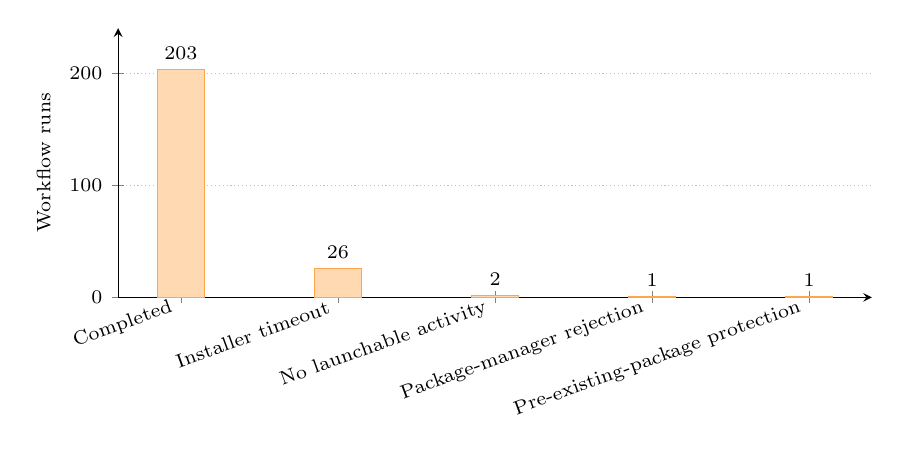
\begin{tikzpicture}
\begin{axis}[
  width=0.92\textwidth, height=5.0cm,
  ybar, bar width=17pt,
  ymin=0, ymax=240,
  ylabel={\scriptsize Workflow runs},
  symbolic x coords={Completed, Installer timeout, No launchable activity, Package-manager rejection, Pre-existing-package protection},
  xtick=data,
  x tick label style={font=\scriptsize, rotate=20, anchor=east},
  y tick label style={font=\scriptsize},
  ymajorgrids, grid style={densely dotted},
  nodes near coords, every node near coord/.append style={font=\scriptsize},
  axis lines=left, enlarge x limits=0.10,
]
% Values match generated-results.tex macros: CompletedWorkflowsN=203,
% FailedDeviceWorkflowsN=30, with the recorded failure classes 26/2/1/1.
\addplot[fill=orange!30, draw=orange!70] coordinates {
  (Completed,203)
  (Installer timeout,26)
  (No launchable activity,2)
  (Package-manager rejection,1)
  (Pre-existing-package protection,1)
};
\end{axis}
\end{tikzpicture}
\caption{Terminal state of every workflow run and the composition of the retained failures. The bars share one denominator of \DevicePackagesN{} package identities; the completed run and the failures are complementary, and the four failure classes sum to the \FailedDeviceWorkflowsN{} retained failures. The last class is simultaneously an uncompleted run and a correct safety behaviour of the runner.}
\label{fig:device-terminal-states}
\end{figure}

The measurement side of the same run is reported separately, because roughly half of the completed workflows have no recorded memory or timing value. The measured subset is therefore reported as a descriptive distribution with its denominator, and the missing values remain missing. They are not replaced by zero, the available subset is never presented without the missing count, and no imputation is used to ``complete'' the series. Because the missingness mechanism has not been identified, the thesis does not claim that the measured subset is a random or unbiased sample of the completed workflows, and it does not assume that the missing values would resemble the measured ones. Two clarifications are required to interpret the two measurements at all. The PSS value describes the launched package's memory after launch; it is not the overhead of the Privacy Lens review engine. The timing value describes the whole recorded workflow; it is not the latency of an individual privacy decision. Repeated operations on the same package identity are not counted as independent device samples.

\section{Temporal Correctness, Restart, and Stress Evidence}

The temporal contribution (C2) is supported by tests written at the abstraction boundary where the claim is made, so that neither the tests nor this chapter silently widens it. Exact-boundary cases exercise timestamps immediately inside and immediately outside a rule-owned window. A six-event fixture is evaluated under all 720 permutations to establish order independence for a fixed subject, pack, effective event multiset, candidate window, and retention set; that qualification matters, because a different arrival order which changes the retained set is not covered by the same result. A seeded 1,000-event burst checks bounded execution rather than presenting a synthetic timing figure as a deployment benchmark. Additional cases verify profile validation, fail-closed rejection of invalid mappings, pack switching, source-receipt generation, integration through the compliance engine, and wording that preserves notification-only behaviour.

Restart behaviour is exercised as a partition, export, restore, and resume comparison rather than as an anecdotal check: for \StressRestartN{} generated cases, the restored temporal evidence receipt must equal the receipt produced by an uninterrupted evaluation. Negative cases reject cross-pack snapshots, expired state, and forged deduplication keys. These results are witnesses inside the stated model. They do not establish completeness against every Android signal, recovery from a corrupted store, or legal accuracy, and the exported ledger is not equivalent to a general history import.

Physical evidence closes a different part of the chain. On 21 August 2026 the then-current source was rebuilt as an offline debug APK and installed by ADB on one OPPO PERM00 device. The UI tree exposed Overview, Findings, and Settings, and the user-visible controlled-device confirmation stated that the fixture was compiled from the active pack, that it was synthetic and advisory, and that it could not inspect or alter another application. Executing it increased the local Findings count from 15 to 16. The new card identified \texttt{\seqsplit{com.zhihengzhang.privacylens.controlled-demo}}, carried the ``Controlled device demo'' provenance label, and rendered the 30-minute, order-agnostic LOCATION, ACTIVITY RECOGNITION, and BODY SENSORS co-occurrence rule once its evidence control was opened. The crash buffer remained empty and the process remained running. This verifies a narrow native-bridge, temporal-engine, ledger, and presentation path. It does not demonstrate a real-world temporal incident, because the fixture neither observed another application nor fabricated sensor activity from the device.

The evidential split is intentional. Automated tests establish temporal rule semantics, mapping substitution, fail-closed behaviour, and non-blocking integration; device inspection establishes installation and one representative interaction path. Neither establishes GDPR compliance, universal Android coverage, legal interpretation, performance on all hardware, or user comprehension.

\subsection{Stress Campaign, Oracle Tier, and Verification Protocol}

To strengthen the evidence beyond the repository corpus, \texttt{\seqsplit{tests/runTemporalStressCampaign.ts}} is executed from a fixed seed over the compiled delivered source. It runs \StressCorpusN{} randomised observation multisets over both registered packs against a count-and-window oracle, \StressRestartN{} random partition, export, restore and resume cases, \StressMalformedN{} malformed-audit cases that require fail-closed rejection with a byte-for-byte unchanged exported temporal ledger, one valid 10,001-entry snapshot that must restore bounded to 10,000 entries, and forged, cross-pack, and expired snapshots that must be rejected. The campaign completes \StressAssertionsN{} assertions and matches the registered temporal rules \StressRuleMatchesN{} times in total, and a stored per-rule breakdown sums exactly to that total over the six registered temporal rules.

Two limits on those figures are stated explicitly rather than left to inference. The assertion count is a count of executed assertions, not of independent samples: it cannot be divided by the corpus size to obtain a population error rate, and it is not decomposable per assertion type from any stored field. The rule-match total is a count of matching events across a generated distribution, not a count of distinct inputs, and it is not a detection rate over the \StressCorpusN{} cases unless per-rule input counts can be shown to be distinct; per-case records were not retained. The generated corpora are therefore counters rather than stored evidence, and a reviewer cannot re-examine an individual case. A non-vacuity guard fails the campaign if any registered temporal rule is never matched, so the corpus cannot silently stop covering one of the rules it declares; the guard covers the registered temporal rules rather than every rule of every pack. Running \texttt{npm run reproduce:thesis-stress} executes the campaign twice and requires both runs to agree on the recorded assertion and rule-match counts before writing a receipt that records the host and the observed totals.

The oracle tier differs between the suites and is named wherever a result is reported. A fixture whose expected value is derived from the same specification that the engine implements yields a conformance result even when the comparison code is written separately, which is the tier of the seeded logical corpus. The temporal rules in the stress campaign are compared against a count-and-window oracle that re-derives counts and windows from each rule's declared requirements instead of calling the production matcher, so its tier is higher within the same model; the oracle nevertheless shares the compiled rule specification, so the comparison is partially independent rather than fully independent. The restart comparison and the order-invariance check are engine-against-engine comparisons of exported receipts, which establishes self-consistency across export, restore, and resume rather than independence from the implementation. Neither tier reaches ecological validity, because the inputs remain generated. Continuous integration runs the enumerated checks from a clean dependency installation, and a release-privacy contract checks that the native controlled method is gated by \texttt{BuildConfig.DEBUG}, with the JavaScript bridge delegating that decision to the native boundary so that an offline debug bundle cannot suppress a valid debug-only test.

Device acceptance remains limited to the actual build, installation, UI tree, screenshot, logcat, and crash-buffer evidence collected for that build. A controlled card is synthetic and cannot be reported as an observed privacy event. Taken together, these results establish reproducibility and the tested fail-closed invariants under the specified generated inputs. They are not a performance benchmark, a proof for every possible input, a legal validation, or field evidence.

\section{Interpretation and Validity}

The final stage asks how much authority the combined evidence supports. It triangulates independent artefacts, examines correlated-oracle risk, interprets metrics, applies the project-defined store-candidate gate, and defines which changes would invalidate the result.

\subsection{Result Boundary}

The evidence supports the claim that the specified code compiles, the rule engine conforms to its fixtures, the Android artefacts build, the final package installs and launches, the main interface renders coherently, and provenance remains visible in the tested workflows. It does not support claims about 24-hour execution, battery cost, memory leaks, unrestricted third-party observation, multiple OEMs, legal compliance, accessibility conformance, production signing, or store acceptance.

\subsection{Evidence Triangulation}

No single method in the campaign was designed to carry the complete acceptance claim. Source inspection is good at confirming constants, branches, labels, and data flow, but it cannot establish which code entered an APK or how a screen rendered. Automated tests execute specified behaviours repeatedly, but their assertions can share assumptions with the implementation. Package inspection observes the assembled artefact, but it cannot prove the meaning of every runtime path. Device interaction observes a concrete installation, but the sample is narrow. The evaluation therefore uses convergence among methods while preserving the scope of each.

Figure~\ref{fig:evaluation-triangulation} presents this assurance structure. Solid arrows connect evidence produced in the study; dashed arrows mark validation that remains external or future. The shape prevents a large logical test count from visually overwhelming the smaller but qualitatively different device, human, and legal evidence classes.

\begin{figure}[H]
\centering
\begin{tikzpicture}[
  node distance=0.55cm,
  evidence/.style={draw, rounded corners, align=center, text width=0.25\textwidth, minimum height=1.25cm, font=\small},
  claim/.style={draw, rounded corners, align=center, text width=0.32\textwidth, minimum height=1.25cm, font=\small},
  arrow/.style={-latex, thick}
]
\node[evidence, fill=blue!7] (source) {Source and rule evidence\\types, branches, fixtures};
\node[evidence, fill=blue!7, right=of source] (tests) {Executed logical evidence\\conformance, adversarial, replay};
\node[evidence, fill=green!9, right=of tests] (package) {Assembled artefact evidence\\APK, AAB, manifest, hashes};
\node[evidence, fill=green!9, below=of package] (device) {Bounded physical evidence\\install, launch, interaction, render};
\node[claim, fill=purple!8, below=of tests] (supported) {Supported engineering claim\\specified behaviour exists in the tested source, package, and device scope};
\node[claim, fill=orange!10, below=of source] (external) {External validation still required\\population usability, accessibility conformance, legal validity, multi-device reliability};
\draw[arrow] (source) -- (tests);
\draw[arrow] (tests) -- (package);
\draw[arrow] (package) -- (device);
\draw[arrow] (tests) -- (supported);
\draw[arrow] (device) -- (supported);
\draw[dashed,-latex,thick] (supported) -- (external);
\end{tikzpicture}
\caption{Evaluation triangulation and claim boundary}
\label{fig:evaluation-triangulation}
\end{figure}

The deterministic tests and source review converge on threshold semantics. Source review identifies the pack-provided baseline, multiplier, daily threshold, burst limit, and source restrictions. Boundary assertions then test values immediately around those decision points. The fixed corpus tests varied inputs at scale. Agreement across these methods reduces the chance that the reported rule differs accidentally from the implemented one. It still does not establish that the rule is a valid legal classifier.

Runtime-boundary tests and presentation tests converge on uncertainty handling. Malformed evidence is rejected at admission, low-context evidence becomes an evidence gap, and presentation projection retains that state. This end-to-end check matters because a correct engine could be undermined if the UI translated an unknown state into reassuring copy. The tests show that selected fixtures preserve meaning through the current projection; screenshot review confirms the principal labels are visible in the rendered flow.

Build logs, output existence, checksums, manifest inspection, installed-package metadata, and physical launch converge on artefact identity. Each closes a different substitution risk. A successful Gradle message without an output file would be insufficient. A local file without a checksum could be confused after rebuilding. Source manifest facts could differ after dependency merging. An installed package could be a stale version. Reading these signals together supports the conclusion that the evaluated handset ran the recorded release candidate.

Visual review and UI-hierarchy inspection also complement each other, because a screenshot shows layout and hierarchy as a person sees them while a hierarchy dump exposes text, bounds and accessibility-node structure; neither replaces screen-reader interaction, large-font testing or participant comprehension.

Triangulation is not vote counting. Where one authoritative check contradicts another, the discrepancy must be resolved rather than outvoted, and greater weight belongs to evidence closest to the released artefact for package claims and to independent human or legal review for substantive claims.

\subsection{Oracle Independence and Correlated Defect Risk}

The main corpus labels are derived from the same published threshold model the implementation is intended to realise. This is appropriate for conformance testing: it asks whether the program implements the specification. It is insufficient for empirical validation because a mistaken specification can yield perfect agreement. The measured 1.0000 precision and recall are therefore implementation-oracle agreement values, not estimates of performance on real legal cases.

Several design choices reduce accidental coupling. The generator records expected polarity directly from its construction, a fresh engine limits cross-case state, boundary cases are written explicitly, and extended tests target properties beyond the main daily-total rule. Nevertheless, developer knowledge shaped both sides. The campaign did not use a separately developed executable oracle, blinded labels, or an external benchmark.

The distinction between what has been done and what has not must be stated precisely here, because a curated campaign of exactly this kind has already been executed. Nine registered, non-equivalent weakenings were applied individually to a copied compilable tree, and the compiled suite failed on every one, as reported above. Three extensions remain \emph{not} done. The first is automatically generated mutants, which would remove the reliance on the author's choice of weakening. The second is independently designed mutants, written by a reviewer who has not read the production engine. The third is property-based generation of many valid and invalid evidence shapes, which would explore inputs beyond the registered corpus while preserving the stated invariants.

Each extension would address a different weakness, and none of them is guaranteed by the 9/9 result. A curated set cannot estimate mutational robustness in general. The registry was revised after the initial execution found candidate weakenings surviving, some of them behaviourally equivalent to the original code and others not witnessed by the cited suite. Because the pre-correction formulations were not retained, the initial set cannot be reconstructed item by item, and this thesis does not report a per-item initial survivor count. The final 9/9 therefore reflects development feedback rather than a blind measure. A detected weakening shows that one assertion distinguishes one wrong implementation; it does not show that unmodelled defects are absent. The same discipline applies in the other direction: a surviving mutant identifies an assertion that executes code without distinguishing correct behaviour, which is a finding about the test suite rather than proof of a program defect.

Two extensions would raise the tier of this evidence: an independently implemented oracle, and ground truth from controlled event traces or independent scenario labelling. Both require work that this thesis does not report, and both are specified as future work in Chapter 7 rather than claimed here.

This distinction explains why the thesis retains the term deterministic corpus rather than benchmark. A benchmark normally suggests comparison against an external reference population. The current corpus is a rigorous regression artefact that protects rule semantics as the code changes. Its value is high, but different from an independently labelled real-world set.

\subsection{Metric Interpretation and Error Analysis}

Precision and recall were included because they expose false-positive and false-negative cells more clearly than accuracy in an imbalanced corpus. The designed 80/20 mixture would allow a trivial always-positive strategy to appear 80 per cent accurate. The full confusion matrix prevents that reading: all 200 controls were negative and all 800 constructed signals were positive under the specified oracle.

The exact totals also make the experiment reproducible. The campaign did not sample a changing external population; it evaluated a fixed generated set. Confidence intervals around the observed proportions would describe repeated sampling from an assumed generator, not uncertainty about the fixed run. More importantly, they would not address specification validity. For this reason the report presents exact agreement and claim boundaries instead of using a narrow interval to imply real-world certainty.

Error analysis remains meaningful even when the main matrix has no disagreements. Adversarial suites reveal categories the primary generator does not represent: unsafe numeric values, prototype-derived identifiers, malformed context, source forgery, temporal overlap, replay, and history isolation. These tests show that corpus size alone is not coverage. A small, carefully targeted case can provide more security evidence than hundreds of additional values drawn from the same safe range.

Reporting for any future field study is specified as future work in Chapters 6 and 7 rather than claimed here: stratification by permission, application category, source authority, foreground status, OEM, Android version and window resolution; inspection of false positives and negatives for common causes; missing acquisition records kept as missing rather than treated as model negatives; excluded cases counted and explained; calibration evaluated separately from discrimination; and denominators defined for operational metrics such as launch success, crash-free periods and rendering smoothness.


\section{Evaluation Synthesis}

The results answer the engineering portion of the research problem question by question rather than as one aggregate score, and Chapter 7 states the answer to each research question. Android evidence connects the accepted source revision to release artefacts, a reconciled manifest, an installed package, and a bounded rendered workflow.

The strongest supported conclusion is therefore a chain rather than a single score. Privacy Lens implements the specified evidence contract, packages that implementation into an installable Android candidate, and communicates its principal limitations coherently on the tested device. Two of the three contributions are carried by that chain: C1 by the preserved evidence and output contract from admission to presentation, and C2 by the bounded temporal, replay, and recovery semantics with their stated conditions and losses. C3 is carried less by any single number than by the way the chain is reported---separate denominators per evidence object, retained failures and missing values, a named oracle tier for each suite, and an explicit statement of what each layer cannot support. The chain stops before legal adjudication, unrestricted acquisition, population performance, broad usability, accessibility conformance, long-run reliability, production signing, and store approval. Chapter 6 examines why those boundaries remain material and which future evidence could move them.
